\chapter[Acceleration of the Alpha-Eigenvalue Rayleigh Quotient Fixed Point Method by Anderson Acceleration][Anderson Acceleration]{Acceleration of the Alpha-Eigenvalue Rayleigh Quotient Fixed Point Method by Anderson Acceleration}
\label{sec:AndAcc}

Like all fixed point methods, the alpha-eigenvalue Rayleigh Quotient Fixed Point method exhibits only linear convergence. In most cases, this rate of convergence is acceptable when other methods are unable to converge the alpha-eigenvalue and eigenvector of interest. However, there exists a set of problems where the alpha-eigenvalue Rayleigh Quotient Fixed Point method converges unacceptably slow. These problems are characterized by large domains where neutrons experience a large amount of scattering before finally being absorbed or leaking out of the domain. For these problems, it might become necessary to use acceleration methods to mitigate slow convergence. In this chapter, we discuss the use of \textit{Anderson acceleration} on the Rayleigh Quotient Fixed Point method for alpha-eigenvalue problems. We examine various slow converging criticality problems of interest and describe the performance of Anderson acceleration. We discuss the reduction in transport sweeps, the associated memory costs of the method, and the practical considerations when using Anderson acceleration.

\section{Anderson Acceleration}

We begin by describing Anderson acceleration. Anderson acceleration originated in the work of Anderson \cite{anderson1965iterative} for the solution of nonlinear integral equations. More recently, work by Walker and Ni \cite{walker_anderson_2011} and Toth and Kelley \cite{toth_convergence_2015} have focused on the use of Anderson acceleration in other applications such as multiphysics problems. 

Consider the fixed point problem
\begin{equation*}
	G(u) = u, \quad G: \mathbb{R}^{N} \rightarrow \mathbb{R}^{N}.
	\label{eq:AAFP}
\end{equation*}
We assume that the iteration converges ($\rho(G'(u^{*})) < 1$) \cite{ostrowski_solution_2016}. Anderson acceleration maintains a history of residuals
\begin{equation}
	f(u) = G(u) - u
\end{equation}
of depth at most $m + 1$, where $m$ is a parameter in the algorithm. An Anderson acceleration iteration that uses $m$ residual histories is referred to as Anderson($m$). Anderson(0) is fixed point iteration by definition. Anderson acceleration for the fixed point problem, Eq.~\ref{eq:AAFP}, is given by Algorithm~\ref{algo:AA1}. 
\begin{algorithm}[!htbp]
	\caption{Anderson Acceleration}
	\label{algo:AA1}
	\begin{algorithmic}
		\STATE{Set $u_{0} =$ an initial guess and $m \geq 1$}
		\STATE{$u_{1} = G(u_{0})$}
		\FOR{$n = 0, 1, 2, \cdots$ until convergence}
			\STATE{Set $m_{n} = \min(m,n)$}
			\STATE{Set $F_{n} = (f_{n-m_{n}}, \cdots, f_{n}),$ where $f_{i} = G(u_{i}) - u_{i}$}
			\STATE{Determine $\alpha^{n} = (\alpha_{0}^{(n)}, \cdots, \alpha_{m_{n}}^{(n)})$ that solves $\min_{\alpha} \norm{F_{n} \alpha^{T}}_{2}$ such that $\sum_{i=0}^{m_{n}} \alpha_{i} = 1$}
			\STATE{Set $u_{n+1} = \sum_{i=0}^{m_{n}} \alpha_{i}^{(n)}G(u_{n-m_{n}+i})$}
			\STATE{Test for convergence}
		\ENDFOR
	\end{algorithmic}
\end{algorithm}

Any norm can be used in the minimization step. However, the $\ell_{2}$ is typically used so that the minimization problem can be formulated as a linear least squares problem \cite{walker_anderson_2011}.

In practice, each $m_{n}$ may be further modified to maintain acceptable conditioning of $F_{n}$. In most applications $m_{n}$ is small. $m_{n} = 1$ or $m_{n} = 2$ is common for large systems due to memory constraints and conditioning requirements.

In the original formulation of Anderson acceleration \cite{anderson1965iterative}, the formulation of the next iterate can be made more general using the expression
\begin{align}
	u_{n+1} &= (1-\beta_{n}) \sum_{i=0}^{m_{n}} \alpha_{i}^{(n)} u_{n-m_{n}+i} + \beta_{n} \sum_{i=0}^{m_{n}} \alpha_{i}^{(n)}G(u_{n-m_{n}+i}) \\
	& = \sum_{i=0}^{m_{n}} \alpha_{i}^{(n)} u_{n-m_{n}+i} + \beta_{n} \bigg (  \sum_{i=0}^{m_{n}} \alpha_{i}^{(n)}G(u_{n-m_{n}+i}) - \sum_{i=0}^{m_{n}} \alpha_{i}^{(n)} u_{n-m_{n}+i} \bigg ),
\end{align}
where $\beta_{n}$ is a relaxation parameter. The relaxation parameters $\beta_{n}$ are usually determined heuristically. In practice, $\beta_{n}$ is a damping parameter ($0 < \beta_{n} \leq 1$) and is used to improve convergence by reducing step lengths when iterates are not near the fixed point solution. Setting $\beta_{n} = 1$ gives the update in Algorithm~\ref{algo:AA1}.

Algorithm~\ref{algo:AA1} requires solving the constrained linear least-squares problem:
\begin{equation}
	min_{\alpha} \norm{F_{n} \alpha^{T}}_{2} \, s.t.\, \sum_{i=0}^{m_{n}} \alpha_{i} = 1.
\end{equation}
Instead, the least squares problem can be formulated \cite{anderson1965iterative} into an equivalent unconstrained problem. This unconstrained Anderson acceleration algorithm is shown in Algorithm~\ref{algo:AA2}.

\clearpage

\begin{algorithm}[!htbp]
	\caption{Unconstrained Anderson Acceleration}
	\label{algo:AA2}
	\begin{algorithmic}
		\STATE{Set $u_{0} =$ an initial guess and $m \geq 1$}
		\STATE{$u_{1} = G(u_{0})$}
		\FOR{$n = 0, 1, 2, \cdots$ until convergence}
			\STATE{Set $m_{n} = \min(m,n)$}
			\STATE{$\Delta F_{n} = (\Delta f_{n-m_{n}}, \cdots, \Delta f_{n-1})$ where $\Delta f_{i} = f_{i+1} - f_{i}$ and $f_{i} = G(u_{i}) - u_{i}$}
			\STATE{Determine $\gamma^{(n)} = (\gamma_{0}^{(n)}, \cdots, \gamma_{m_{n}-1}^{(n)})$ that solves $\min_{\gamma} \norm{f_{n} - \Delta F_{n} \gamma^{T}}_{2}$}
			\STATE{Set $u_{n+1} = G(u_{n}) - \sum_{i=0}^{m_{n}-1} \gamma_{i}^{(n)} \Delta g_{n - m_{n} + i}$ with $\Delta g_{i} = G(u_{i+1}) - G(u_{i})$}
			\STATE{Test for convergence}
		\ENDFOR
	\end{algorithmic}
\end{algorithm}
Determining the coefficients $\gamma^{(n)} = (\gamma_{0}^{(n)}, \cdots, \gamma_{m_{n}-1}^{(n)})$ is done by a QR factorization
\begin{equation}
	\Delta F_{n} = Q_{n}R_{n},
\end{equation}
\begin{equation}
	R_{n} \gamma^{(n)} = Q_{n}^{T}f_{n}.
\end{equation}
The need for a QR factorization increases the computation cost of one iteration of Anderson acceleration. However, various fast and inexpensive QR factorization methods are available. Despite the increased cost per iteration, if Anderson acceleration substantially reduces the number of iterations required for convergence then this cost may be acceptable.

It is usually desirable to do multiple fixed point iterations before beginning acceleration. Doing fixed point iterations may allow the vector iterates to get closer to the region of convergence of the fixed point. This is easily implementable in the Anderson acceleration algorithms by prescribing the number of fixed point iteration evaluations to be done before starting the acceleration.

It is Algorithm~\ref{algo:AA2} that is applied to the acceleration of the alpha-eigenvalue Rayleigh Quotient Fixed Point method.

\section{Anderson Acceleration of Slowly Converging Alpha-Eigenvalue Rayleigh Quotient Fixed Point Problems}

In this section we consider various critical slab problems that are slow to converge using the alpha-eigenvalue Rayleigh Quotient Fixed Point method. These problems are characterized by long slab widths and high amounts of scattering. Since the alpha-eigenvalue is related to the time it takes for a neutron to be absorbed or leak out of the system, the wide slabs with many scattering interactions require many transport sweeps to converge. We apply Anderson acceleration to these problems and explore the performance of the acceleration method for various parameters of the method. We look at the effects of the number of residual vectors used in the calculation of the next iterate, the number of initial fixed point iterations done before beginning acceleration, and the impacts of the relaxation parameter $\beta_{n}$.

\subsection{Uranium-Heavy Water Critical Slab (Sood Criticality Benchmark Problem 73)}

\begin{table}[!htbp]
	\caption{Two-Group U-D$_{2}$O Problem Cross Sections (cm$^{-1}$)}
	\label{table:D2O-Sood73}
	\begin{subtable}[!htbp]{1.0\textwidth}
		\centering\ra{1.3}
		\begin{tabular}{@{}cccccc@{}}\toprule
			$g$ & $\sigma_{g} $ & $\nu_{g}$ & $\sigma_{fg}$ & $\chi_{g}$ & $v_{g}$ [cm/s] \\ 
        			\midrule
			1 & 0.33588  & 2.50 & 0.002817 & 1.0 & 2.0 \\
			2 & 0.54628  & 2.50 & 0.097 & 0.0 & 1.0 \\
			\bottomrule
		\end{tabular}
	\caption{U-D$_{2}$O(73) Cross Sections}
	\end{subtable}%
	\vspace{0.25cm}
	\begin{subtable}[!htbp]{1.0\textwidth}
	\centering\ra{1.3}
	\begin{tabular}{@{}ccc@{}}\toprule
	$g' \rightarrow g$ & 1 & 2 \\ 
        \midrule
	1 & 0.31980 & 0.004555   \\
	2 & 0.0 & 0.42410  \\
	\bottomrule
	\end{tabular}
	\caption{U-D$_{2}$O(73) Scattering Block-$\sigma_{s0}$}
	\end{subtable}
		\begin{subtable}[!htbp]{1.0\textwidth}
	\centering\ra{1.3}
	\begin{tabular}{@{}ccc@{}}\toprule
	$g' \rightarrow g$ & 1 & 2 \\ 
        \midrule
	1 & 0.06694 & -0.0003972 \\
	2 & 0.0 & 0.05439  \\
	\bottomrule
	\end{tabular}
	\caption{U-D$_{2}$O(73) Scattering Block-$\sigma_{s1}$}
	\end{subtable}
\end{table}

\begin{table}[!htbp]
\caption{Sood Criticality Problem 73 Critical Width and Reference Alpha-Eigenvalue \cite{sood2003analytical}}
	\label{table:Sood73Ref}
	\begin{subtable}[h]{1.0\textwidth}
	\centering\ra{1.3}
	\begin{tabular}{@{}ccc@{}}\toprule
	Cross Section Set & r$_{c}$ [cm] & Calculated $\alpha$ [s$^{-1}$] \\
	\midrule
	U-D$_{2}$O(73) & 1000.506133 & $-1.221913 \times 10^{-5}$ \\
	\bottomrule
	\end{tabular}
	\end{subtable}%
\end{table}

\begin{table}[!htbp]
\caption{Anderson Acceleration Performance for Sood Criticality Problem 73 ($\beta_{n} = 1, M = 50, L = 16$)}
	\label{table:Sood73AA}
	\begin{subtable}[h]{1.0\textwidth}
	\centering\ra{1.3}
	\begin{tabular}{@{}ccc@{}}\toprule
	Anderson($m_{n}$) & Calculated $\alpha$ [s$^{-1}$] & Transport Sweeps \\
	\midrule
	Anderson(0) & $-1.221913 \times 10^{-5}$ & 22749 \\
	Anderson(1) & $-1.221913 \times 10^{-5}$ & 17620 \\
	Anderson(2) & $-1.221913 \times 10^{-5}$ & 4814  \\
	Anderson(3) & $-1.221913 \times 10^{-5}$ & 2777  \\
	Anderson(4) & $-1.221913 \times 10^{-5}$ & 1854  \\
	Anderson(5) & $-1.221913 \times 10^{-5}$ & 6008  \\
	\bottomrule
	Initial Fixed Point Iterations = 0
	\end{tabular}
	\end{subtable}%
	\vspace{0.25cm}
	\begin{subtable}[h]{1.0\textwidth}
	\centering\ra{1.3}
	\begin{tabular}{@{}ccc@{}}\toprule
	Anderson($m_{n}$) & Calculated $\alpha$ [s$^{-1}$] & Transport Sweeps \\
	\midrule
	Anderson(1) & $-1.221913 \times 10^{-5}$ & 17775 \\
	Anderson(2) & $-1.221913 \times 10^{-5}$ & 9204 \\
	Anderson(3) & $-1.221913 \times 10^{-5}$ & 2583 \\
	Anderson(4) & $-1.221913 \times 10^{-5}$ & 1407 \\
	Anderson(5) & $-1.221913 \times 10^{-5}$ & 6172 \\
	\bottomrule
	Initial Fixed Point Iterations = 5
	\end{tabular}
	\end{subtable}%
	\vspace{0.25cm}
	\begin{subtable}[h]{1.0\textwidth}
	\centering\ra{1.3}
	\begin{tabular}{@{}ccc@{}}\toprule
	Anderson($m_{n}$) & Calculated $\alpha$ [s$^{-1}$] & Transport Sweeps \\
	\midrule
	Anderson(1) & $-1.221913 \times 10^{-5}$ & 12186 \\
	Anderson(2) & $-1.221913 \times 10^{-5}$ & 11382 \\
	Anderson(3) & $-1.221913 \times 10^{-5}$ & 4809 \\
	Anderson(4) & $-1.221913 \times 10^{-5}$ & 2626 \\
	Anderson(5) & $-1.221913 \times 10^{-5}$ & 3603 \\
	\bottomrule
	Initial Fixed Point Iterations = 10
	\end{tabular}
	\end{subtable}
\end{table}

\begin{table}[!htbp]\ContinuedFloat
	\begin{subtable}[h]{1.0\textwidth}
	\centering\ra{1.3}
	\begin{tabular}{@{}ccc@{}}\toprule
	Anderson($m_{n}$) & Calculated $\alpha$ [s$^{-1}$] & Transport Sweeps \\
	\midrule
	Anderson(1) & $-1.221913 \times 10^{-5}$ & 12241 \\
	Anderson(2) & $-1.221913 \times 10^{-5}$ & 3604  \\
	Anderson(3) & $-1.221913 \times 10^{-5}$ & 6713  \\
	Anderson(4) & $-1.221913 \times 10^{-5}$ & 5430  \\
	Anderson(5) & $-1.221913 \times 10^{-5}$ & 2925  \\
	\bottomrule
	Initial Fixed Point Iterations = 20
	\end{tabular}
	\end{subtable}%
	\vspace{0.25cm}
	\begin{subtable}[h]{1.0\textwidth}
	\centering\ra{1.3}
	\begin{tabular}{@{}ccc@{}}\toprule
	Anderson($m_{n}$) & Calculated $\alpha$ [s$^{-1}$] & Transport Sweeps \\
	\midrule
	Anderson(1) & $-1.221913 \times 10^{-5}$ & 17166 \\
	Anderson(2) & $-1.221913 \times 10^{-5}$ & 7363 \\
	Anderson(3) & $-1.221913 \times 10^{-5}$ & 4205 \\
	Anderson(4) & $-1.221913 \times 10^{-5}$ & 1729 \\
	Anderson(5) & $-1.221913 \times 10^{-5}$ & 2253 \\
	\bottomrule
	Initial Fixed Point Iterations = 50
	\end{tabular}
	\end{subtable}%
	\vspace{0.25cm}
	\begin{subtable}[h]{1.0\textwidth}
	\centering\ra{1.3}
	\begin{tabular}{@{}ccc@{}}\toprule
	Anderson($m_{n}$) & Calculated $\alpha$ [s$^{-1}$] & Transport Sweeps \\
	\midrule
	Anderson(1) & $-1.221913 \times 10^{-5}$ & 17313 \\
	Anderson(2) & $-1.221913 \times 10^{-5}$ & 14811 \\
	Anderson(3) & $-1.221913 \times 10^{-5}$ & 10654 \\
	Anderson(4) & $-1.221913 \times 10^{-5}$ & 3923 \\
	Anderson(5) & $-1.221913 \times 10^{-5}$ & 3657 \\
	\bottomrule
	Initial Fixed Point Iterations = 100
	\end{tabular}
	\end{subtable}
\end{table}

\begin{figure}[!htbp]
\centering
\begin{subfigure}{\textwidth}
  \centering
  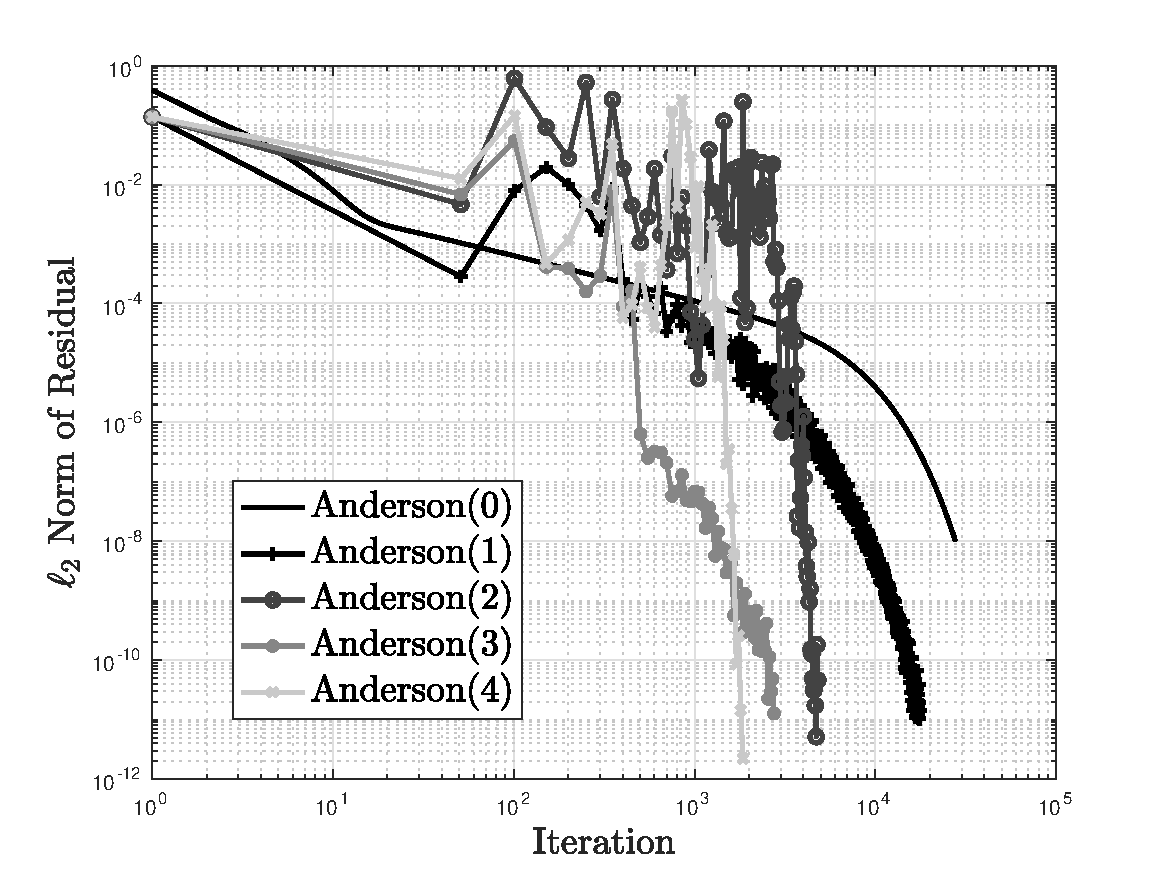
\includegraphics[width=.9\linewidth]{Figures/AndersonAcceleration/SoodProb73}
\end{subfigure}
\caption{Anderson Acceleration Convergence for Sood Criticality Problem 73 ($\beta_{n} = 1$)}
\label{fig:AASoodProb73}
\end{figure}


